\documentclass[12pt]{article}
\usepackage[pdftex]{graphicx}
\usepackage{amsfonts}
\usepackage[italian]{babel}
\usepackage{graphicx}
\usepackage{color}
\usepackage{multirow,bigdelim}

\definecolor{grey}{rgb}{0.3,0.3,0.3}

\usepackage{listings, framed}
\lstset{
  language=Java,
  showstringspaces=false,
  columns=flexible,
  basicstyle={\small\ttfamily},
  frame=none,
  numbers=none,
  keywordstyle=\bfseries\color{grey},
  commentstyle=\itshape\color{red},
  identifierstyle=\color{black},
  stringstyle=\color{blue},
  numberstyle={\ttfamily},
%  breaklines=true,
  breakatwhitespace=true,
  tabsize=3,
  escapechar=|
}

%****************enlarge layout
\textheight     243.5mm
\topmargin      -20.0mm
\textwidth      480pt
\hoffset        -80pt
%*****************theorems and such
\newcounter{esnu}
\newenvironment{esercizio}{\medskip \noindent {\bf Esercizio\addtocounter{esnu}{1} \arabic{esnu}}}{}
\pagestyle{empty}
\newcommand{\liff}{\mathrel{\leftrightarrow}}   % Logical IFF Symbol
\newcommand{\metaiff}{\Longleftrightarrow}      %iff in metatheory

\begin{document}

%\begin{tabular}{llclcr}
% \hspace{-35pt} &{\bf COGNOME:} & \hspace{100pt}        &{\bf NOME:}    & \hspace{100pt}        &{\bf MATRICOLA:}%\hspace{35pt} \\
%\hline
%\end{tabular}
\begin{center} {\bf Esame di Programmazione II, 26 settembre 2019}\end{center}
%\`

\emph{
Si crei un progetto Eclipse e, nella directory dei sorgenti,
si crei il package \texttt{it.univr.graph}. Si copi al suo interno
le classi \texttt{Graph.java} e \texttt{Main.java}.
}

\emph{
Se si realizzano nuove classi, le si crei dentro
il package \texttt{it.univr.graph}.
Non si modifichi le dichiarazioni dei metodi. Si possono definire altri campi,
metodi, costruttori e classi, ma devono essere \texttt{private}.
La consegna fornita compila.
Anche la soluzione che verr\`a consegnata dovr\`a compilare,
altrimenti non verr\`a corretta.
}
\mbox{}\\

\begin{esercizio}~\textbf{[20 punti, si consegni \texttt{Graph.java}]}
  Si completi la classe \texttt{Graph.java}, che implementa un grafo diretto.
  Un grafo contiene la lista dei
  suoi nodi e ciascun nodo contiene il suo valore (di tipo generico \texttt{E})
  e la sua \emph{stella uscente}, cio\`e la lista dei nodi a cui \`e connesso,
  senza ripetizioni. I nodi posso essere normali o colorati di rosso
  e questo nell'implementazione viene rappresentato dalle classi interne
  \texttt{Node} e \texttt{RedNode}.
  Un grafo nasce senza nodi, che si possono poi aggiungere con il metodo
  \texttt{add} (per i nodi normali) e \texttt{addRed} (per i nodi rossi).
  Archi fra nodi dello stesso grafo si possono aggiungere con il loro metodo \texttt{linkTo}.
  Un grafo \`e iterabile, quindi il suo metodo \texttt{iterator()}
  deve restituire un iteratore dei nodi del grafo.
  Infine, con il metodo \texttt{toString}
  \`e possibile avere una rappresentazione testuale del grafo
  in formato dot. Per esempio, il seguente grafo di stringhe:
  %
  \begin{center}
    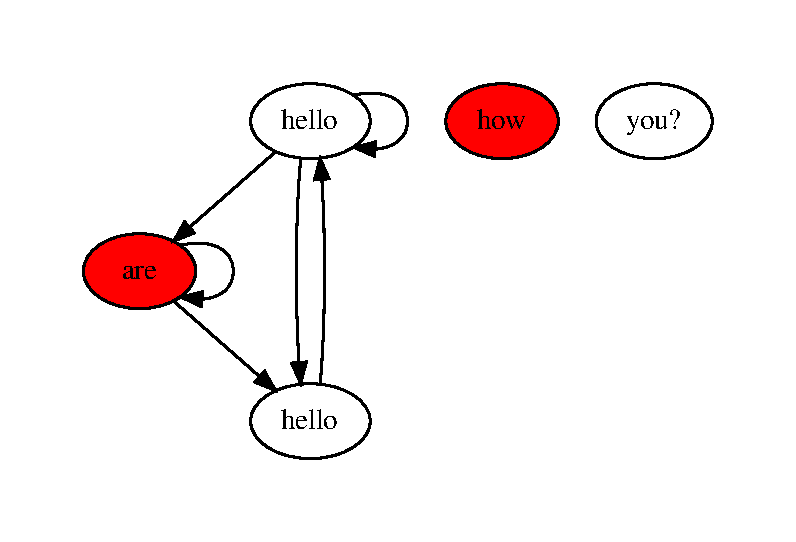
\includegraphics[width=10cm]{g1.pdf}
  \end{center}
  %
  dovrebbe avere il seguente risultato per \texttt{toString}, che rispetta la sintassi
  del formato dot:
\begin{verbatim}
digraph {
  node0 [label="hello"]
  node0 -> node0
  node0 -> node2
  node0 -> node4
  node1 [label="how", style="filled", fillcolor="red"]
  node2 [label="are", style="filled", fillcolor="red"]
  node2 -> node2
  node2 -> node4
  node3 [label="you?"]
  node4 [label="hello"]
  node4 -> node0
}
\end{verbatim}
%
Nel formato dot i nodi vengono dichiarati con nome e valore (\texttt{label})
e gli archi sono rappresentati come frecce. I nodi rossi hanno uno stile
riempito (\texttt{filled}) in rosso.
La scelta dei nomi dei nodi dentro la stampa in dot \`e irrilevante.
L'importante \`e che i nomi siano diversi per nodi diversi.
Nell'esempio sopra si \`e usato \texttt{node0}, \texttt{node1} ecc.,
ma ogni altra scelta \`e valida.
\end{esercizio}

\begin{esercizio}~\textbf{[11 punti, si consegni \texttt{Main.java}]}
  Si completi la classe \texttt{Main.java} in modo che il suo metodo \texttt{main}
  \begin{enumerate}
  \item costruisca e stampi in dot il grafo di stringhe della pagina precedente;
  \item costruisca e stampi in dot il seguente grafo di \texttt{java.lang.Integer}:
    %
    \begin{center}
      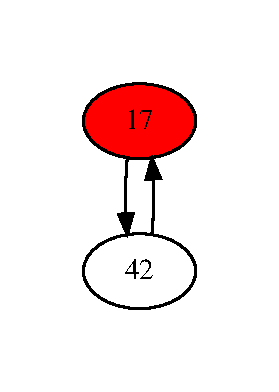
\includegraphics[width=3.5cm]{g2.pdf}
    \end{center}
    %
  \item costruisca un grafo di stringhe contenente un unico nodo con valore
    \texttt{"hello"}, provando poi a legarlo a un nodo del primo grafo, il che
    dovrebbe generare un'eccezione.
  \end{enumerate}
\end{esercizio}
\vspace*{1ex}
\hrule
\mbox{}\\
\emph{Se tutto \`e  corretto, l'esecuzione del \texttt{Main} dovrebbe stampare:}
\begin{verbatim}
digraph {
  node0 [label="hello"]
  node0 -> node0
  node0 -> node2
  node0 -> node4
  node1 [label="how", style="filled", fillcolor="red"]
  node2 [label="are", style="filled", fillcolor="red"]
  node2 -> node2
  node2 -> node4
  node3 [label="you?"]
  node4 [label="hello"]
  node4 -> node0
}

digraph {
  node0 [label="17", style="filled", fillcolor="red"]
  node0 -> node1
  node1 [label="42"]
  node1 -> node0
}

Exception in thread "main" java.lang.IllegalArgumentException:
   Cannot link nodes from distinct graphs
\end{verbatim}

\end{document}
